\section{Background}
\label{sec:background}

\subsection{Meteorological Background}

You need to find some sources indicating weather convective or frontal precipitation is the main source of extreme precipitation on the different durations. 

Explain convention and what generally causes the most extreme precipitation on the different durations. Present some typical precipitation values at the selected durations values?

Maybe the GEO4902 work can be included here in the background? Or it can be included as a separate section to highlight problems with forecasting extreme events? This can also be used to justify why we have to choose the maximum values from multiple grid.boxes around the respective station.   
one paper under AROME folder also highlights what effect horizontal resolution have on extreme precipitation. 

\subsubsection{Precipitation}
precipiation formation processes: collision and coalecence, ice crystal, cloud seeding. Convective, frontal, orographic. Stbility. Summer and winter. 
Precipitation is often categorized by the physical process creating it and may vary on both spatial and temporal scale. One can often relate the precipitation process to the relationship between the vertical and the horizontal extent, where the vertical velocity can be related to these two. The temporal scale varies from minutes to days, and the the spatial scale varies from hundreds of meters to hundreds of kilometers. Large-scale precipitation events are typically on a synoptic scale, characterized by a horizontal dimension many times greater than the vertical extent. Hence, the vertical velocity is often small in theses systems. Smaller-scale systems have shorter horizontal extent and often vertical extent equal to or almost equal to the vertical. In these systems the vertical speed is often large compared to large-scale systems. Normally precipitation is separated into three main categories; stratiform, orographic and convective precipitation.

\subsubsubsection{Large-scale}
some on this? at least mention somewhere what types of precipitation events usually causes the largest extremes for differnt durations. From 0-3 hours its typically convective precipitation, but when you are getting closer to a full day it might as well be large-scale stratiform precipitation. 
\subsubsubsection{orographic}
some on this?
\subsubsubsection{Convective Precipitation}
Convective precipitation originates from clouds driven by convection. These clouds are cumulus-type clouds forming in an unstable atmosphere as warm air rises due to buoyancy forces. The vertical extent is determined by the depth of the unstable layer and its degree of instability. The cumulus clouds are distinct in their shape with a flat base and a "cotton-like" appearance. They can also be observed with narrow, towering plumes on top. Horizontally the extent is typically around 3 km, while the initial thermal in which condensation first occurs can be only tens of meters. Typically the lifetime of cumulus clouds are from a few minutes to hours. If the persist for many hours they also tend to grow substantially in size. The horizontal and vertical extent is comparable, but a cumulus cloud can under right conditions (\textbf{do i need to elaborate further on this?}) develop to a cumulonimbus cloud reaching all the way to the top of the stratosphere \cite{rogers}. Once the recognizable anvil-shaped cumulonimbus is formed it is very likely to produce rain, thunder and lightning. Although cumulus clouds are commonly associated with nice weather, as the convection it self typically occurs due to the sun heating the ground during daytime in summer creating buoyant air, once the rising parcel of air becomes saturated condensation will occur and precipitation will form. As the warm and moist air rises it cools to the point where the air is saturated on water vapour. Once condensation begins, latent heat is released and precipitation forms.

maybe include some schematics on buoyancy and instability? also the dry and wet adiabat and stability criteria? 

\begin{figure}[hbt!]
    \centering
    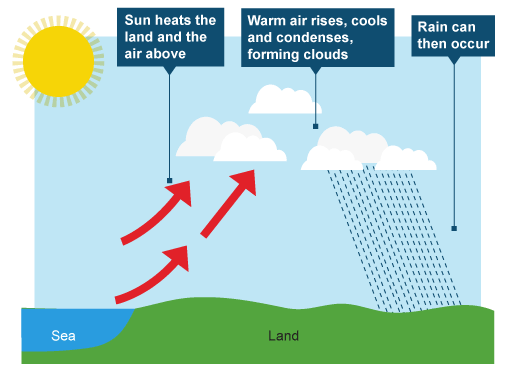
\includegraphics[scale=0.4]{figures/convection-rain.png}
    \caption{Schematic Convection. From: https://anessoriginal.wordpress.com/elective-geog/variable-weather-and-changing-climate-a-continuing-challenge/key-question-1-wc/1-convectional-rain/.
    \cite{convection}}
    \label{fig:convection}
\end{figure}


Given the short temporal scale and the small horizontal scale the convective precipitation, also known as showers, are rather local phenomena you can watch form and propagate past your neighbourhood. Events at such small scales proves hard to capture for climate models, and even operational forecasting are far from spot on with predicting the where and the when of these events. 

\begin{figure}[hbt!]
    \centering
    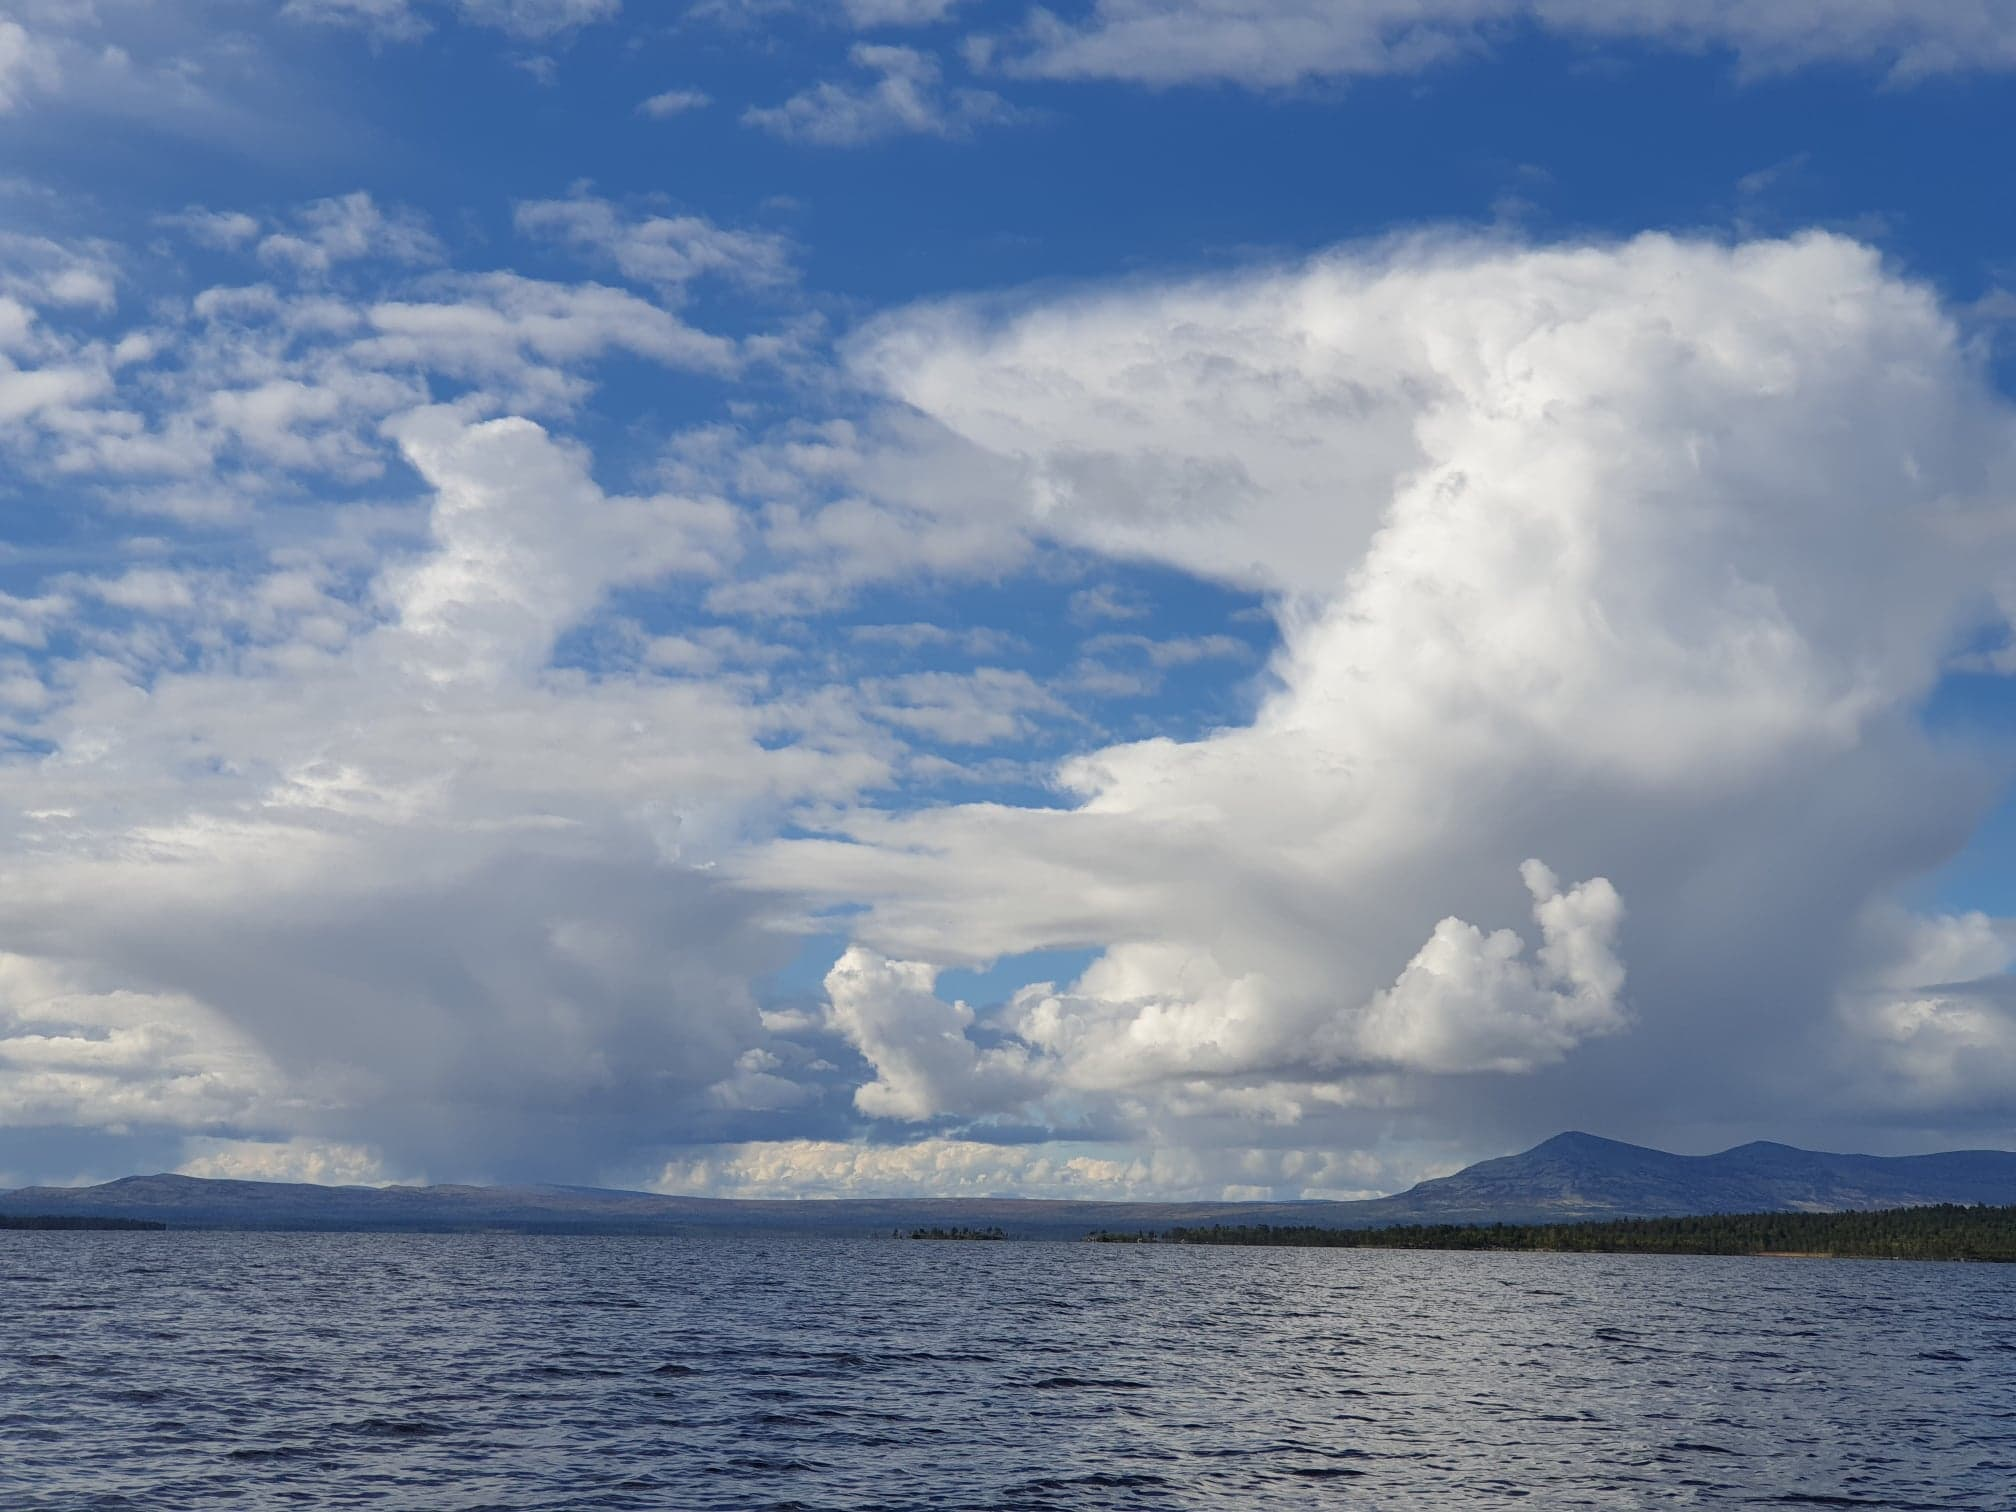
\includegraphics[scale=0.2]{figures/cumulus_bilde.jpg}
    \caption{Formation of convective Cumulus clouds over land in Femundsmarka, Norway.
    \cite{cumulus}}
    \label{fig:cumulus}
\end{figure}

\subsubsection{Convection}

\subsubsection{Dry convection}

Convection is often treated as an adiabatic process. This is a thermodynamic process in which no heat or mass is transferred between the system in question and the surroundings. However, energy can be transferred from the system to the surroundings through work. Being a compressible fluid the density of the atmosphere is a function of both temperature and pressure; $\rho = \rho(p,T)$. Furthermore it obeys the perfect gas law, and $\rho = p/RT$. As a parcel rises from an initial height $z_1$ it moves into an environment of lower pressure at height $z_2$, adjusting to this pressure by expanding along the way. This expansion exerts work on the environment, making the parcel cool. To determine the buoyancy of the parcel at $z_2$ one must know the evolution of the parcel temperature between $z_1$ and $z_2$.

Considering a parcel of ideal gas of unit mass with a volume V. Using the first law of thermodynamics,

\begin{equation}
    \delta Q = dU + dW
    \label{1law}
\end{equation}
where $\delta Q$ is an amount of heat exchange with the surroundings, $dU$ is the change in energy and $dW$ is the change in external work. Eq. \eqref{1law} can be written as 

\begin{equation}
    \delta Q = c_vdT + pdV
    \label{1law2}
\end{equation}

where $c_cdT$ is the change in internal energy due to change in temperature $dT$ and $pdV$ is the work done by the parcel on its surroundings by expanding an amount $dV$. $c_v$ is specific heat at constant volume. Rewriting Eq. \eqref{1law2} with repeated use of $p=\rho RT$ yields 

\begin{equation}
    \delta Q = c_pdT - \frac{dp}{\rho}
    \label{thermo1}
\end{equation}

where $c_p = R + c_v$ is specific heat at constant pressure. 

For adiabatic processes $\delta Q = 0$, thus

\begin{equation}
    c_pdT = \frac{dp}{\rho}
    \label{dq0}
\end{equation}

The hydrostatic balance,

\begin{equation}
    \frac{\partial p}{\partial z} +g\rho = 0
\end{equation}

describes how pressure decreases with height in proportion with the weight of the overlying atmosphere. Using the hydrostatic equation and assuming $p \simeq p_{e}$, for a small upward displacement in Eq.\eqref{dq0} the parcel`s temperature under an adiabatic displacement will change according to

\begin{equation}
    \frac{dT}{dz} = -\frac{g}{c_p} = - \Gamma_d
    \label{drylaps}
\end{equation}

where $\Gamma_d$ is called the dry adiabatic lapse rate and the notation $e = environment$. Now if the parcel is displaced from $z_1$ to $z_2$ it will experience a restoring force depending on the density of the environment. At $z_2$ the environment has temperature $T_2 \simeq T_1 + (dT/dz)_e \delta z$ where $(dT/dz)_e = \Gamma_e$ is the environmental lapsrate, pressure $p_2$ and density $\rho_2 = p_2/RT_2$. The parcel has temperature $T_P = T_1 - \Gamma_d\delta z$, pressure $p_2$ and density $\rho_P = p_2/RT_P$. Depending on whether $T_P$ is greater than, equal to or less than $T_2$ the parcel will be positively, neutrally or negatively buoyant. Thus, criterion for stability can be written

\begin{equation}
    \begin{rcases}
      \text{Unstable}\\
      \text{Neutral}\\
      \text{Stable}
    \end{rcases}   
    \text{if} \left(\frac{dT}{dZ}\right)_e = \Gamma_e 
    \begin{cases}
      < - \Gamma_d \\
      = - \Gamma_d \\
      > - \Gamma_d
    \end{cases}
    \label{stabcond}
\end{equation}

From Eq. \eqref{stabcond} a compressible atmosphere is unstable if temperature decreases with height faster than the adiabatic laps rate. Given $c_p = 1005 Jkg^{-1}K^{-1}$ in Eq. \eqref{drylaps} $\Gamma_d \simeq 10 K km^{-1}$. Typically the dry laps rate decreases from around 6,5 $K km^{-1}$ at low latitudes to around 4.5 $K km^{-1}$ at polar latitudes \ref{lapsrate}. Thus, no dry convection is expected and the atmosphere can generally be considered stable to dry convection.     

\textbf{must describe the unknowns where they are first mentioned}

\subsubsubsection{Moist convection}

Since the atmosphere is normally stable in the absence of condensation most convection in the atmosphere is moist convection. If a moist air parcel is lifted it cools adiabatically, and if it is cooled enough to saturate some water vapor condenses to form a cloud. Once saturated to parcel releases latent heat, adding buoyancy to the parcel and thus increasing the instability.
Moisture of air is often expressed as specific humidity 

\begin{equation}
    q = \frac{\rho_v}{\rho}
\end{equation}

This is the ratio of mas of water to the mass of air er unit volume. Q is conserved given no mixing. The saturation-specific humidity, $q_*$, is the specific humidity at which saturation occurs. $q_*$ can be written:

\begin{equation}
    q_* = \frac{\frac{e_s}{R_v T}}{\frac{p}{RT}} = \left(\frac{R}{R_v}\right)\frac{e_s}{p}
    \label{qnote}
\end{equation}

where $e_s$ is saturated partial pressure of water vapor. 

Implicitly this means that $q_*$ is a function of both temperature and pressure. Lifting a parcel would decrease the pressure and cool the parcel. This alone would make q* increase with altitude, but the exponential dependence of es on T counteracts this effect, making the q* decrease rapidly with altitude. Thus a moist parcel usually do not have to rise a lot before it reaches the condensation level Zc where $q>q_*$. At this point and above excess water vapor will condensate creating a visible cloud. The cloud will extend up in the atmosphere until neutral buoyancy. As the parcel rises latent heat is released, resulting in a slower decrease of temperature with height compared to the dry adiabatic as rate.  Thus, a warmer or moister air parcel will result in a taller cloud compared to drier or cooler air. While the temperature of the parcel changes according to the dry adiabatic laps rate below the cloudbase, it follows the saturated adiabat upwards from $z_c$. 

When condensation occurs there will be a release of latent heat in the amount $\delta Q = -L dq$ where $L$ is latent heat of condensation and $dq$ is change in specific humidity $q$. For an air parcel undergoing moist adiabatic displacement one can insert this into \eqref{thermo1} to get 

\begin{equation}
    c_p dT = \frac{dp}{\rho}-L dq
    \label{adlap}
\end{equation}

Assuming hydrostatic balance of the environment, $dp/\rho = -gdz$ gives

\begin{equation}
    d(c_pT + gz + Lq) = 0
\end{equation}

where $c_pT+gz$ is the dry static energy and $Lq$ is the latent heat content. Combined these two terms are called the moist static energy. Furthermore, since the parcel is always saturated $q$ can be replaced by $q_*$ in Eq.\eqref{adlap}, and since $q_*=q_*(p,T)$ now

\begin{equation}
    dq_* = \frac{\partial q_*}{\partial p}dp + \frac{\partial q_*}{\partial T}dT
    \label{dqnote}
\end{equation}

Inserting Eq. \eqref{qnote} in Eq. \eqref{dqnote} yields 

\begin{equation}
        \frac{\partial q_*}{\partial p} = -(\frac{R}{R_v})\frac{e_s}{p^2} = -\frac{q_*}{p}
        \label{qfracp}
\end{equation}
and
\begin{equation}
            \frac{\partial q_*}{\partial T} = (\frac{R}{R_v})\frac{1}{p}\frac{de_s}{dT} = (\frac{R}{R_v})\frac{\beta e_s}{p} = \beta q_*
            \label{qfracT}
\end{equation}

where $\beta e_s = de_s/dT$. Combining Eq. \eqref{qfracp}, Eq. \eqref{qfracT} and Eq. \eqref{adlap} with some rearranging yields

\begin{equation}
    -\frac{dT}{dz} = \Gamma_s = \Gamma_d \left[\frac{1+Lq_*/RT}{1+\beta Lq_*/c_p} \right]
\end{equation}

$\Gamma_s$ is called the saturated adiabatic lapse rate. The term inside the brackets are always less than unity, making $\Gamma_s < \Gamma_d$. However, at high latitudes $q_*$ becomes very small, making them close to equal. The qualitative impact on condensation is evident; release of latent heat within a rising parcel makes it warmer and thus more buoyant, destabilizing the atmosphere, that is if

\begin{equation}
    \frac{dT}{dz} < -\Gamma_s
\end{equation}

where $\Gamma_s < \Gamma_d$ \cite{marshall}. 
\textbf{this is conditional stability, dont know if I need to elaborate on this}


\subsubsection{Types and location of convection}



\subsection{Area}

The area investigated in this thesis is Oslo, the capitol of Norway. This location is selected for a number of reasons. Firstly there are multiple stations in the area witch have long, high quality data series of precipitation. This is essential because it allows for comparison to the modeled IDF values. When analysing IDF curves short time series is a problem in it self, therefore having multiple high quality data series is very valuable to the analysis. Also, multiple stations covering a rather small area like in this case may highlight certain features in the IDF curves related to topography or other mechanisms influencing precipitation that would otherwise have been hidden. Secondly the Oslo area is a typical urban area, making it vulnerable to short duration extreme precipitation. Improving the knowledge on extreme precipitation events may potentially save the area and its population for large weather-related costs in the future. Another reason for selecting this area was the availability of processed data. Data from the selected stations had been cleaned and checked for analysis beforehand as part of the \textbf{Julia paper (how do I address this?)}. 

\subsection{Data}
\subsubsection{Measurements}
Precipitation measurements used in this project is obtained from pluviometers operated by the Norwegian Water Resources and Energy Directorate (NVE) or the respective municipalities in corporation with  MET Norway. Since the late 1990s and early 2000s the operating pluviometer has been the Lambrecht 1518H3 tipping bucket pluviometer manufactured by the German company Lambrecht meteo GmbH \cite{lutz_idf}. The Lambrecht pluviometer has a measuring range of 0.1 mm precipitation at time resolution of 1 minute and a given accuracy of $\pm$ 2$\%$. Intensity correction is done to account for loss of rain due to the time required for the bucket to tip. MET Norway supervised the installation of the pluviometers and ensured installation according to the recommendations from the World Meteorological Organization (WMO). Additionally MET Norway performed quality control and storage on all data from the pluviometers. Before the now operational Lambrecht some of the stations operated with the Norwegian produced pluviograph Plumatic, manufactured by Kongsberg Våpenfabrikk A/S. It was replaced partially due to is lack of heating, making it operational only in the extended summer months, from mid-April to mid-October. The Lambrecht also suffers from poorer data quality during winter due to snowcaps or ice-slush obstruction spite been heated.  

The proposed method in this study requires annual maxima for each duration as input, thus a requirement for season completeness is necessary. The requirement where here set to at least 80\% of the days throughout the season covered and of good quality. Hence the precipitation series extracted where shorter than the total operational period for all stations. The number of extracted years with annual maxima is found in Table \textbf{number of table below}. Lutz et al 2020 analysed monthly precipitation for 1,2 and 3 hours in two locations in Oslo and found that the highest occurrence of short-duration, high-intensity precipitation was during the summer months. In combination with lack of high-quality data during the winter period, especially from before the 1990s when the Plumatic pluviometer were still in use, makes the extended summer period, 1st of May to 30th of September, best suited for the IDF analysis in this study. Furthermore, time series of 10 years is here considered to be an absolute minimum for calculation of IDF values. The twelve stations listed in Table \textbf{table under, need numer} are the ones left meeting these criteria in the municipality of Oslo.   

\\

\begin{center}
\begin{tabular}{ |p{3cm}||p{3cm}|p{3cm}|p{3cm}|  }[hbt!]
\hline
\multicolumn{4}{|c|}{Oslo Stations} \\
\hline
 Station Name & Station NR & Years AM & Operational From\\
 Ljabruveien & 17980  & 17 &  01.01.1985-\\
 Lambergseter & 18020 & 25 & 15.05.1999-\\
 Hovin & 18210 & 17 & 15.01.1999-\\
 Haugenstua & 18269 & 15 & 01.01.2000-\\
 Vestli & 18270 & 32 & 18.04.1974-\\
 Hausmannsgt & 18320 & 20 & 21.06.1984-04.11.2013\\
 Disen & 18420 & 20 & 02.06.1998-\\
 Vestre Vika & 18640 & 13 & 22.05.1974-03.10.1998\\
 Blindern PLU & 18701 & 48 & 16.04.1968-\\
 Bygdøy & 18815 & 16 & 01.01.2000-\\
 Besserud & 18920 & 13 & 29.09.2998-\\
 Lilleaker & 18980 & 13 & 01.01.2000-   
\end{tabular}
\end{center}

\textbf{the section "measurements" in Lutz et al., 2020 has the description of the station data. Essentially annual maxima for each duration and station.} Tipping bucket pluviometers does not function properly during winter, so this is basically summer-data. Time series of 10 years is concidered an asolute minimum here, hence the choice of these 12 stations (you can also include the two from Bærum if you get the data). 

\subsubsection{AROME model and data}

For this study precipitation output from the non-hydrostatic Applications of Research to Operations at Mesoscale (AROME)\cite{seity_arome} model have been used. The model is developed by Météo-France and is operated by a cooperative effort named Meteorological Cooperation on Operational Numerical Weather Prediction (MetCoOp) between the Norwegian Meteorological Institute (MET-Norway) and the Swedish Meteorological and Hydrological Institute (SMHI). AROME is used operationally for high-resolution numerical weather prediction (NWP) since 2008 and has recently been used in a climate-configuration for long-term climate simulations \cite{lind_arome]}. Being one of the first long-term climate simulations on regional convection-permitting (\<4km)scales for the Scandinavian region this data-set provides added opportunities for analysis of extreme precipitation.  
\\
\\
HARMONIE-Climate cycle 38 (HCLIM38) on 3 km resolution with explicit deep convection is the parenting model used in the this study (Lindstedt et al. 2015\cite{lindstedt_hclim}; Lind et al. 2016\cite{lind_hclim}). A comprehensive description of the model system is presented in Belušić et al.(2020)\cite{belusic_hclim}. The model proved strong improvement on representation of precipitation compared to similar model-setups with coarser models in Lind et al. 2020 \cite{lind_arome}. Most evident was the improvement in reduction of "drizzle" and increased occurrence of high intensity precipitation events in addition to better timing and amplitude of the diurnal cycle. The simulations was conducted within the Nordic Convection Permetting Climate Projections project (NorCP), which is one of the leading projects on increasing knowledge of climate changes and processes over the Fenno-Scandinavian region. Here the model-run with the AROME physics package is applied. AROME (Bengtsson et al. 2017)\cite{bengtsson_arome} is designed for convection-permitting scales and non-hydrostatic dynamics with 65 vertical layers. The boundary state for HCLIM38-AROME (HCLIM3) is obtained from the global ERA-Interim reanalysis (Berrisford et al. 2011)\cite{erai}. This data has a horizontal grid of approximately 80 km, available every 6 hour. An alternative set of boundary data from EC-Earth (ECE) is also applied, providing a slightly different climate simulation.    
ECE
\\
HCLIM3
surface and precip representation

\cite{lind_arome} citation figure arome domain 
\begin{figure}[hbt!]
    \centering
    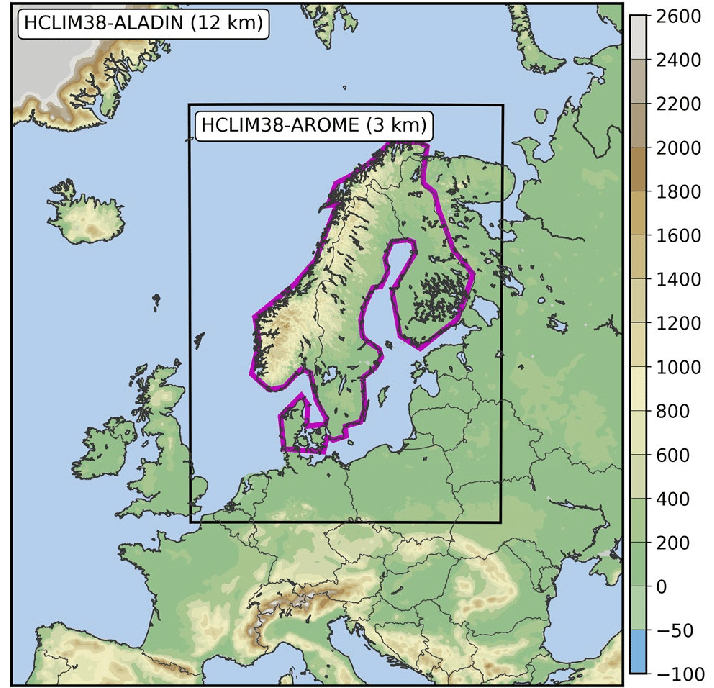
\includegraphics[scale=0.4]{figures/arome_domain.png}
    \caption{Domain used for HCLIM38-ALADIN (12km) simulation and domain used for HCLIM38-AROME (3km) simulation in the inner black rectangle. The colorscale represents the altitude above mean sea level in meters, and the magent colored area defines the Fenno-Scandinavian region. Source: Lind et al. 2020 \cite{lind_arome}}
    \label{fig:arome_domain}
\end{figure}

\subsubsection{AROME: difficulties with convective forecasting, an example}

MÜller et al. 2017 \cite{muller} highlights the challenge of precise precipitation forecasting of convective cells. Even though the precipitation amount may be well-forecasted it can be fatal for decision-makers if it is mislocated with a few kilometers. Here a case study illustrating this challenge is presented. 

7nt of August 2019 15:00-18:00 UTC a heavy rainfall event occurred in Bærum, Norway. According to a METinfo report \ref{metreport} the event caused local damage, clogged drainage systems and numerous flooded basements. The forecast prior to the event revealed unstable air masses with strong vertical movement throughout southern Norway. Besides an elevated KAPE-index north-west of where the event actually occurred there where little indication for such an event in the Bærum-area. During the event several records for short-duration precipitation was set at the Gjettum station in Bærum: 36,5mm/30min, 47,9mm/1h and 61,3/3h. These recordings have returnperiods of >200 years, >100 years and >50 years respectively. The 24-h accumulated precipitation forecast is produced as a 10-member ensemble mean. The ensemble mean forecast in Figure \ref{fig:ens_mean} show some precipitation in the area west of Bærum with magnitude of around 2 mm/24h.  

\begin{figure}[hbt!]
    \centering
    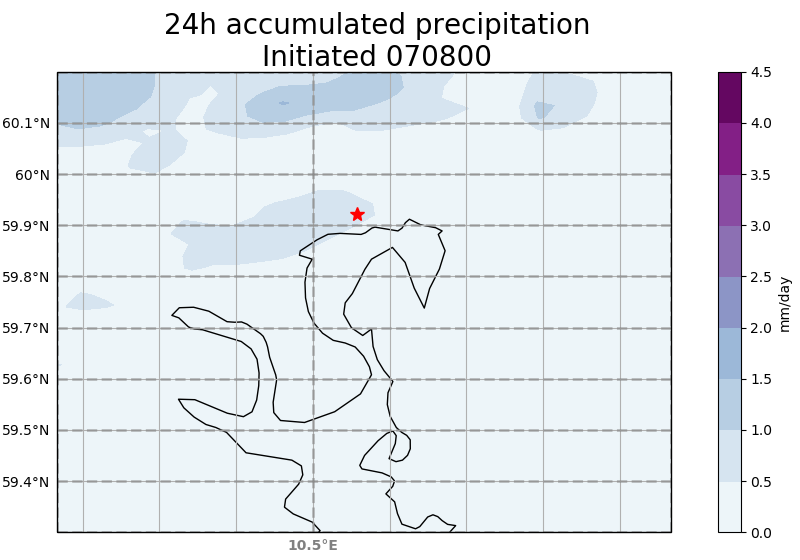
\includegraphics[scale=0.4]{figures/ens_mean.PNG}
    \caption{24-h ensemble mean precipitation forecast initiated 7th of August 2019 00:00 UTC. The black line is the shoreline in the Oslofjord, Norway. The red star marks the location of the Bærum station.}
    \label{fig:ens_mean}
\end{figure}

Ensemble members different realizations of the model, each with a slightly different set of initial conditions. Even though the ensemble mean forecast shows no signs of extreme precipitation the individual members may reveal some red flags. All members are equally a realization of the model, which highlights the uncertainty of the precipitation forecasting within AROME. In Figure \ref{fig:ensmember} two ensemble members show two very different forecasts. One seems to capture the localization and partly the amount of the event quite well while the other predicts no precipitation at all. 

\begin{figure}[hbt!]%
    \centering
    \subfloat[\centering Ensemble member 1]{{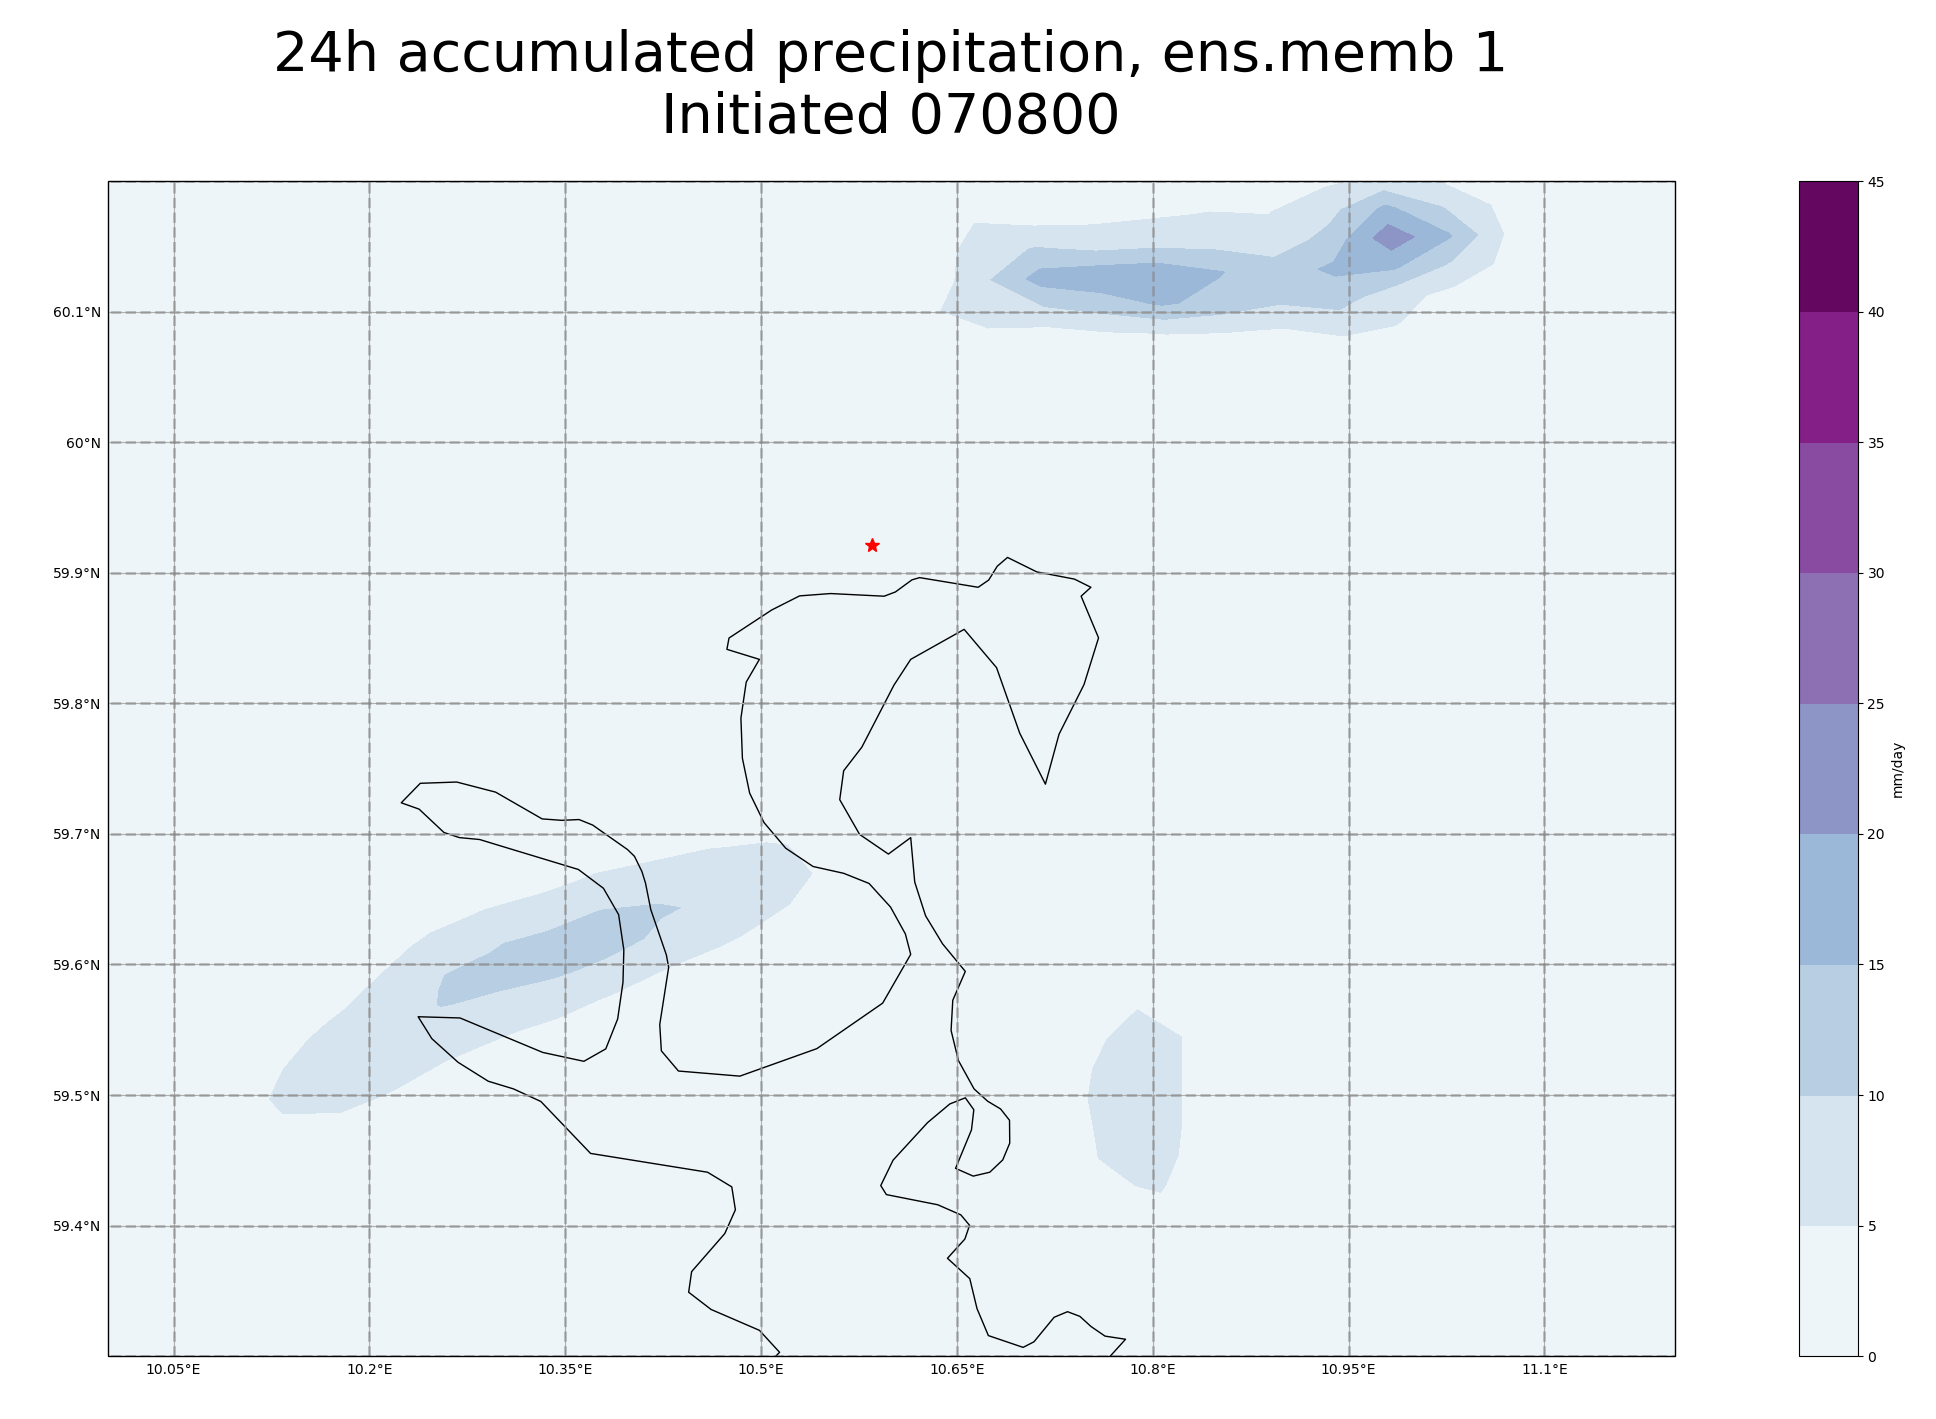
\includegraphics[width=5.5cm]{figures/ens1.PNG} }}%
    \qquad
    \subfloat[\centering Ensemble member 4 ]{{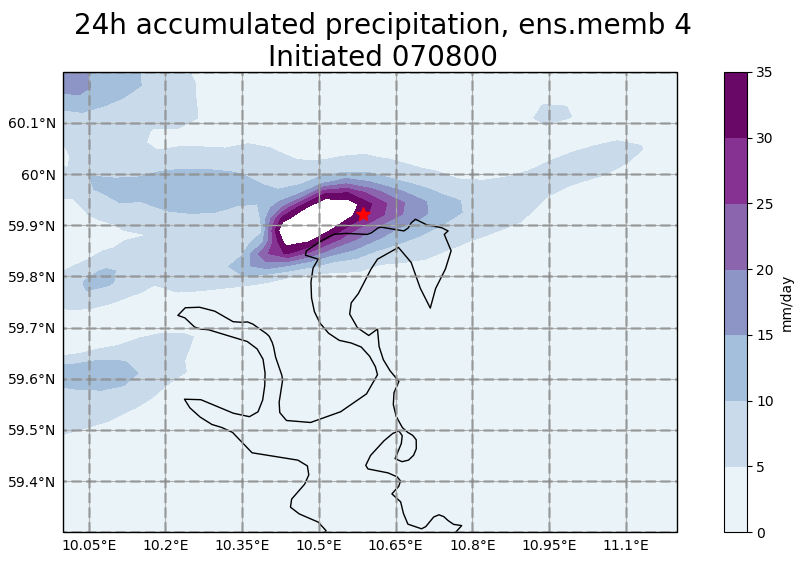
\includegraphics[width=5.5cm]{figures/ens4.PNG} }}%
    \caption{Two ensemble members from the 24-h accumulated preciptiation forecast initiated 7th of August 2019 at 00:00. The red star marks the Bærum station.}%
    \label{fig:ensmember}%
\end{figure}

this case study is also usefull to highlight how the various ensemble members dissagree, and in a way represent different verions of the reality. This is comparable to the climate model and can be used as a pro to why the periods does not have to match exactly.  
\section{Method}

There are several ways to extract annual maxima from the precipitation data. In the following paragraph the different methods used on this study will be presented.  
\subsection{Annual Maxima}

The methods used to extract annua maxima from the precipitation data-series. 
Common:
From this time-series the annual maxima is extracted for each duration, making a data-series with maximum values with length n equal to number of years.  Something more here or add this to all of them?

\begin{enumerate}

\item 1grid 
Hereafter named “1GRID”. Select gridpoint closest to the respective station. A sliding filter for each duration is applied, building a timeseries with summed values for each timestep. From this time-series the annual maxima is extracted for each duration, making a data-series with maximum values with length n equal to number of years. 

\item 9grid
Hereafter named “9GRID”. Select the gridpoint closest to the respective station and the neighbouring gridpoints following a 3x3 pattern. A sliding filter for each duration is applied, building a timeseries with summed values for each timestep. The filter select the maximum value out of the 9 gridpoints for each timestep. Thus a resulting precipitation value for a given duration may consist of precipitation values from different gridpoints. 

\item 9mean
Hereafter named “9MEAN”. Select the gridpoint closest to the respective station and the neighbouring gridpoints following a 3x3 pattern. A sliding filter for each duration is applied, building a timeseries with summed values for each timestep. The filter select the maximum value for each of the 9 gridpoints, making 9 time-series with annual maximum values for each duration. The mean annual maximum of the 9 is then calculated. 

\item 9max
Hereafter named “9MAX”. Select the gridpoint closest to the respective station and the neighbouring gridpoints following a 3x3 pattern. A sliding filter for each duration is applied, building a timeseries with summed values for each timestep. The filter select the maximum value for each of the 9 gridpoints, making 9 time-series with annual maximum values for each duration. The max annual maximum of the 9 is then calculated.

\end{enumerate}

Comparison of the methods: 
1GRID is a plain selection method compared to the other methods. The initial reason for using other methods was that 1GRID was underestimating the resulting IDF-curves compared to the station-based curves for almost all stations and durations. 9GRID is designed to be an optimal selection method is the sense that the absolute maximum values possible for the area as an entity is chosen. This method is artificial compared to the others because a maximum value for any given duration may consist of precipitation values from different gridpoints, where the next maximum value may consist of entirely different gridpoint values.    

